\documentclass[12pt]{beamer}
\newenvironment{ConCodigo}[1]
  {\begin{frame}[fragile,environment=ConCodigo]{#1}}
  {\end{frame}}
\graphicspath{{Imagenes/}{../Imagenes/}}
\usepackage[utf8]{inputenc}
\usepackage[spanish]{babel}
\usepackage{hyperref}
\usepackage{etex}
%\reserveinserts{28}
\usepackage{amsmath}
\usepackage{amsthm}
\usepackage{mathtools}
\usepackage{multicol}
\usepackage{multirow}
\usepackage{tabulary}
\usepackage{booktabs}
\usepackage{nccmath}
\usepackage{physics}
\usepackage{biblatex}
\usepackage[outdir=./]{epstopdf}
%\epstopdfsetup{outdir=./}
\usepackage{graphicx}
%\usepackage{enumitem,xcolor}
\usepackage{siunitx}
%\sisetup{scientific-notation=true}
%\usepackage{fontspec}
\usepackage{lmodern}
\usepackage{float}
\usepackage[format=hang, font=footnotesize, labelformat=parens]{caption}
\usepackage[autostyle,spanish=mexican]{csquotes}
\usepackage{standalone}
\usepackage{blkarray}
\usepackage{algorithm}
\usepackage{algorithmic}
\usepackage{tikz}
\usepackage[siunitx, RPvoltages]{circuitikz}
\usetikzlibrary{arrows,patterns,shapes}
\usetikzlibrary{decorations.markings}
\usetikzlibrary{arrows}
\usepackage{color}
\usepackage{xcolor}
%\usepackage{beton}
%\usepackage{euler}
%\usepackage[T1]{fontenc}
\usepackage[sfdefault]{roboto}  %% Option 'sfdefault' only if the base font of the document is to be sans serif
\usepackage[T1]{fontenc}
\renewcommand*\familydefault{\sfdefault}
\DeclareGraphicsExtensions{.pdf,.png,.jpg}
\usepackage{hyperref}
\renewcommand {\arraystretch}{1.5}
\newcommand{\python}{\texttt{python}}
\usefonttheme[onlymath]{serif}
\setbeamertemplate{navigation symbols}{}
\usetikzlibrary{patterns}
\usetikzlibrary{decorations.markings}
\tikzstyle{every picture}+=[remember picture,baseline]
%\tikzstyle{every node}+=[inner sep=0pt,anchor=base,
%minimum width=2.2cm,align=center,text depth=.15ex,outer sep=1.5pt]
%\tikzstyle{every path}+=[thick, rounded corners]
\setbeamertemplate{caption}[numbered]
\newcommand{\ptm}{\fontfamily{ptm}\selectfont}
%Se usa la plantilla Warsaw modificada con spruce
\mode<presentation>
{
  \usetheme{Warsaw}
  \setbeamertemplate{headline}{}
  \useoutertheme{default}
  \usecolortheme{albatross}
  \setbeamercovered{invisible}
}
% \AtBeginSection[]
% {
% \begin{frame}<beamer>{Contenido}
% \normalfont\mdseries
% \tableofcontents[currentsection]
% \end{frame}
% }

\input{../Preambulos/pre_codigo}
\makeatletter
\setbeamertemplate{footline}
%\setbeamercolor{title in head/foot}{fg=Green}
{
  \leavevmode%
  \hbox{%
  \begin{beamercolorbox}[wd=.333333\paperwidth,ht=2.25ex,dp=1ex,center]{author in head/foot}%
    \usebeamerfont{author in head/foot} \textcolor{white}{\insertsection}
  \end{beamercolorbox}}%
  \begin{beamercolorbox}[wd=.333333\paperwidth,ht=2.25ex,dp=1ex,center]{title in head/foot}%
    \usebeamerfont{title in head/foot} \textcolor{white}\insertsubsection
  \end{beamercolorbox}%
  \begin{beamercolorbox}[wd=.333333\paperwidth,ht=2.25ex,dp=1ex,right]{date in head/foot}%
    \usebeamerfont{date in head/foot} \textcolor{white}\insertshortdate{}\hspace*{2em}
    \textcolor{white}\insertframenumber{} / \textcolor{white}\inserttotalframenumber\hspace*{2ex} 
  \end{beamercolorbox}}%
  \vskip0pt%
\makeatother
\normalfont
\usepackage{ccfonts}% http://ctan.org/pkg/{ccfonts}
\usepackage[T1]{fontenc}% http://ctan.or/pkg/fontenc
\renewcommand{\rmdefault}{cmr}% cmr = Computer Modern Roman
\linespread{1.3}
\title{Ecuaciones diferenciales parciales}
\subtitle{Curso de Física Computacional}
\author{M. en C. Gustavo Contreras Mayén}
\setbeamercolor{background canvas}{bg=blue!15}
\setbeamercolor{section in toc}{fg=blue}
\setbeamercolor{subsection in toc}{fg=blue!85}
\setbeamercolor{normal text}{fg=black}
\setbeamercolor{frametitle}{fg=white}
\captionsetup{font=scriptsize,labelfont=scriptsize}
\newcommand{\funcionazul}[1]{\textcolor{blue}{\textbf{\texttt{#1}}}}
\newcommand{\textoazul}[1]{\textcolor{blue}{#1}}
\usepackage{totcount}
\regtotcounter{section}
\usepackage{multido}

\newcommand{\mytableofcontents}[0]{
\multido{\I=1+1}{\totvalue{section}}{
  \begin{frame}<beamer>
  \setcounter{section}{\I}
  \frametitle{Outline}
  \tableofcontents[
    currentsection,
    sectionstyle=show/show,
    subsectionstyle=show/show/hide,
  ]
  \end{frame}
}
\setcounter{section}{0}
}

\begin{document}
\maketitle
\fontsize{14}{14}\selectfont
\spanishdecimal{.}

\mytableofcontents

%\begin{frame}{Contenido}
%\tableofcontents[pausesections]
%\end{frame}
\section{EDP Parabólicas}
\frame{\tableofcontents[currentsection, hideothersubsections]}
\subsection{Introducción EDP Parabólicas}
\begin{frame}
\frametitle{Ecuación para el desarrollo}
Como prototipo de una EDP de tipo parabólico, podemos utilizar  la ecuación de difusión en 1D o la ecuación de calor.
\\
\bigskip
Las técnicas de discretización aplicadas y el análisis de estabilidad correspondiente tienen validez general y son aplicables también a otras ecuaciones parabólicas.
\end{frame}
\begin{frame}
\frametitle{Consideraciones importantes}
A pesar del considerable número de soluciones analíticas disponibles para la ecuación de difusión, éstas se limitan a geometrías simples y coeficientes de difusión constantes.
\end{frame}
\begin{frame}
\frametitle{Consideraciones importantes}
Las condiciones de frontera manejables analíticamente son igualmente simples, sin embargo, las soluciones se expresan a menudo como series infinitas, que no son triviales para evaluar.
\end{frame}
\begin{frame}
\frametitle{Consideraciones importantes}
Para obtener soluciones de la ecuación de difusión que modelen de manera realista las situaciones prácticas, generalmente se necesita recurrir a algoritmos numéricos.
\end{frame}
\begin{frame}
\frametitle{Consideraciones importantes}
Básicamente, éstos implican restringir la solución a un conjunto discreto de puntos de malla y aproximar las derivadas por esquemas de diferencias finitas con relación a éstos.
\\
\bigskip
Posteriormente, el enfoque numérico se reduce a resolver el sistema lineal resultante, cuyas incógnitas son los valores de la solución en los puntos de malla.
\end{frame}
\subsection{Ecuaciones de difusión y calor 1D}
\begin{frame}
\frametitle{Ecuaciones de difusión y calor 1D}
\begin{align}
\dfrac{\partial u}{\partial t} - D \: \dfrac{\partial^{2} u}{\partial x^{2}} &= 0
\label{eq:ecuacion_13_36} \\
\dfrac{\partial u}{\partial t} - K \: \dfrac{\partial^{2} u}{\partial x^{2}} &= f(x, t)
\label{eq:ecuacion_13_37}
\end{align}
describen la evolución temporal y la distribución espacial de la concentración de un elemento difusor $(u (x, t) \equiv c (x, t))$ y la temperatura del sistema $(u (x, t) \equiv T(x,t))$, respectivamente.
\end{frame}
\begin{frame}
\frametitle{Ecuaciones de difusión y calor 1D}
El coeficiente de difusión $D$, relaciona el flujo difusivo $J_{\text{\tiny{dif}}}$, con el gradiente de concentración por la ley de Fick, mientras que la difusividad térmica $K$, relaciona el flujo de calor $J_{\text{\tiny{calor}}}$, con el gradiente de temperatura por la ley de Fourier:
\[ J_{\text{\tiny{dif}}} = - D \: \dfrac{\partial c}{\partial x} \hspace{1cm}  J_{\text{\tiny{calor}}} = - K \: \dfrac{\partial T}{\partial x} \]
La expresión anterior de la ecuación de calor también preveé una fuente de calor $f(x, t)$
\end{frame}
\begin{frame}
\frametitle{Ecuaciones de difusión y calor 1D}
A pesar de que ambas ecuaciones parecen estar espacialmente en 1D, de manera alternativa se puede asumir que modelan una geometría en un plano 3D, en una \enquote{losa}.
\end{frame}
\begin{frame}
\frametitle{Ecuaciones de difusión y calor 1D}
En la que existe una dependencia explícita sólo en la coordenada cartesiana perpendicular a la losa ($x$ en las ecuaciones anteriores) y no hay dependencia de las otras dos coordenadas ($y-z$), a lo largo de las cuales la extensión del sistema se considera implícitamente infinita.
\end{frame}
\begin{frame}
\frametitle{Condiciones iniciales y de frontera}
Modelar una situación física en particular requiere, además de la EDP real, que se proporcionen las condiciones iniciales y de frontera.
\end{frame}
\begin{frame}
\frametitle{Condiciones iniciales}
Las condiciones iniciales especifican la solución sobre todo el dominio espacial en un momento inicial $t_{0}$:
\begin{equation}
U(x, t_{0}) = u^{0} (x), \hspace{1cm} x \in [0, L]
\label{eq:ecuacion_13_38}
\end{equation}
\end{frame}
\begin{frame}
\frametitle{Condiciones de frontera}
Las CDF definen el comportamiento de la solución en la frontera para $t > t_{0}$.
\\
\bigskip
Por simplicidad, consideraremos para un tiempo dado, las CDF de tipo Dirichlet, que implican valores de solución en las fronteras:
\begin{equation}
u(0, t) = u_{0}^{0}, \hspace{1cm} u(L, t) = u_{L}^{0}
\label{eq:ecuacion_13_39}
\end{equation}
\end{frame}
\begin{frame}
\frametitle{Discretización de la ED parabólicas}
Hay varios métodos manuales para discretizar ecuaciones parabólicas.
\\
\bigskip
No obstante, con ligeras modificaciones de los esquemas de discretización se tiene un impacto considerable en la estabilidad y exactitud de la evolución temporal de la solución.
\end{frame}
\section{Métodos de diferencias finitas}
\frame{\tableofcontents[currentsection, hideothersubsections]}
\subsection{Tres enfoques de diferencias finitas}
\begin{frame}
\frametitle{Métodos de diferencias finitas}
A continuación, abordamos tres enfoques de diferencias finitas:
\setbeamercolor{item projected}{bg=red!70!black,fg=white}
\setbeamertemplate{enumerate items}[circle]
\begin{enumerate}[<+->]
\item El método explícito.
\item El método implícito.
\item El método de Crank-Nicolson.
\end{enumerate}
\end{frame}
\begin{frame}
\captionsetup{font=scriptsize,labelfont=scriptsize}
\begin{figure}
	\centering
	\includestandalone[scale=0.8]{mallaSolucionEDP_05}
	\caption{Configuración de nodos espaciales y temporales para tres métodos de discretización de EDP parabólicas.}
\end{figure}
\end{frame}
\subsection{Método explícito de diferencias finitas}
\begin{frame}
\frametitle{Método explícito de diferencias finitas}
Comenzaremos la discretización para la ecuación de difusión (\ref{eq:ecuacion_13_36}) junto con las CDF (\ref{eq:ecuacion_13_38}) y (\ref{eq:ecuacion_13_39}), haciendo una malla espacio-temporal regular, caracterizada por los nodos:
\begin{align}
x_{i} &= (i - 1) \; h_{x}, \hspace{1cm} i = 1, 2, \ldots, N_{x} \label{eq:ecuacion_13_40} \\
t_{n} &= n \; h_{t}, \hspace{1.8cm} n = 0, 1, 2, \ldots \label{eq:ecuacion_13_41}
\end{align}
donde $h_{t}$ es el paso temporal y $h_{x}$ representa el paso entre los $N_{x}$ nodos espaciales.
\end{frame}
\begin{frame}
\frametitle{Método explícito de diferencias finitas}
El espaciamiento de los nodos está dado por
\begin{equation}
h_{x} = \dfrac{L}{N_{x} - 1}
\label{eq:ecuacion_13_42}
\end{equation}
\end{frame}
\begin{frame}
\frametitle{Método explícito de diferencias finitas}
La primera derivada con respecto al tiempo $\partial u / \partial t$ en el nodo espacio - temporal $(x_{i}, t_{n})$ puede obtenerse de una manera directa a partir de la aproximación lineal de la serie de Taylor con respecto a $t$ para la constante $x = x_{i}$
\[ u_{i}^{n + 1} = u_{i}^{n} + h_{t} \; \left( \dfrac{\partial u}{\partial t} \right)_{i,n} + O(h_{t}^{2}) \]
donde $u_{i}^{n} \equiv u(x_{i}, t_{n})$
\end{frame}
\begin{frame}
\frametitle{Método explícito de diferencias finitas}
Separando la derivada temporal, se obtiene el esquema de diferencias hacia adelante:
\begin{equation}
\left( \dfrac{\partial u}{\partial t} \right)_{i,n} = \dfrac{u_{i}^{n + 1} -u_{i}^{n}}{h_{t}} + O(h_{t})
\label{eq:ecuacion_13_43}
\end{equation}
\end{frame}
\begin{frame}
\frametitle{Método explícito de diferencias finitas}
El carácter \enquote{hacia adelante} se da por la presencia de la solución propagada de $t^{n + 1}$ en la expresión de la derivada en $t^{n}$, mientras que el hecho de que el esquema mantenga sólo el primer orden exacto en $h_{t}$ se debe a la división implícita por $h_{t}$.
\end{frame}
\begin{frame}
\frametitle{Método explícito de diferencias finitas}	
Para la segunda derivada espacial en el nodo espacio - temporal $(x_{i}, t_{n})$, podemos usar el esquema de diferencias centrales:
\begin{equation}
\left( \dfrac{\partial^{2} u}{\partial x^{2}} \right)_{i,n} = \dfrac{u_{i + 1}^{n} - 2 \: u_{i}^{n} + u_{i - 1}^{n}}{h_{x}^{2}} + O(h_{x}^{2})
\label{eq:ecuacion_13_44}
\end{equation}
Que involucra sólo la información de $t_{n}$ y de los puntos espaciales ubicados simétricamente alrededor del nodo donde se está calculando la derivada.
\end{frame}
\begin{frame}
\frametitle{Método FTCS}
Sustituyendo las expresiones de diferencias finitas (\ref{eq:ecuacion_13_43}) y (\ref{eq:ecuacion_13_44}) en la ecuación de difusión (\ref{eq:ecuacion_13_36}), se obtiene el \emph{método espacio - temporal hacia adelante} (\textcolor{blue}{Forward Time Central Space FTCS})
\begin{equation}
\dfrac{u_{i}^{n + 1} - u_{i}^{n}}{h_{t}} =  D \; \dfrac{u_{i + 1}^{n} - 2 \: u_{i}^{n} + u_{i - 1}^{n}}{h_{x}^{2}}
\label{eq:ecuacion_13_45}
\end{equation}
\pause
que prorporciona una aproximación del orden $O(h_{x}^{2} + h_{t})$ para la ecuación de difusión en el nodo espacio - temporal $(x_{i}, t_{n})$
\end{frame}
\begin{frame}
\frametitle{Método FTCS}
Por lo que podemos expresar la solución propagada en el siguiente paso temporal $t_{n + 1}$ para cada punto interior $x_{i}$ de la malla espacial, sólo en términos de valores previos de tiempo anterior $t_{n}$:
\begin{equation}
u_{i}^{n + 1} = \lambda \: u_{i - 1}^{n} + (1 - 2 \lambda) \: u_{i}^{n} + \lambda \: u_{i + 1}^{n} \hspace{0.5cm} i = 2, 3, \ldots, N_{x} -1
\label{eq:ecuacion_13_46}
\end{equation}
donde
\begin{equation}
\lambda = \dfrac{D \: h_{t}}{h_{x}^{2}}
\label{eq:ecuacion_13_47}
\end{equation}
\end{frame}
\begin{frame}
\frametitle{Método FTCS}
En cuanto a los valores de la solución en la frontera, están fijos por las condiciones de Dirichlet (\ref{eq:ecuacion_13_39}) a lo largo de la propagación y no requieren ningún tratamiento particular:
\begin{equation}
u_{1}^{n + 1} = u_{1}^{n} = u_{0}^{0}, \hspace{1cm} u_{N_{x}}^{n + 1} = u_{N_{x}}^{n} = u_{L}^{0}
\label{eq:ecuacion_13_48}
\end{equation}
\end{frame}
\begin{frame}
\frametitle{Método FTCS}
Puesto que en cada paso del tiempo, los componentes de la solución propagada pueden expresarse independientemente de la ec. (\ref{eq:ecuacion_13_46}), exclusivamente basada en los datos del paso de tiempo previo.
\end{frame}
\begin{frame}
\frametitle{Proceso de propagación}
Se dice que el \textoazul{método FTCS es explícito} si consideramos el proceso de propagación, al re-escribir la ec. (\ref{eq:ecuacion_13_46}) a la ec. (\ref{eq:ecuacion_13_48}) en notación matricial
\begin{equation}
\mathbf{u}^{n + 1} =  \mathbf{B} \cdot \mathbf{u}^{n}, \hspace{1cm} n = 1, 2, \ldots
\label{eq:ecuacion_13_49}
\end{equation}
\end{frame}
\begin{frame}
\frametitle{Proceso de propagación}
La matriz de propagación $\mathbf{B}$ es tridiagonal y el vector $\mathbf{u}^{n}$ recoge los valores de solución de todos los puntos de malla espacial en el paso de tiempo $t_{n}$:
\fontsize{12}{12}\selectfont
\begin{equation}
\mathbf{B} = \begin{bmatrix}
1 & 0 & & & 0 \\
\lambda & 1 - 2 \lambda & \lambda & & & \\
 & \ddots & \ddots & \ddots & \\
 & & \lambda & 1 - 2 \lambda & \lambda \\
 0 & & & 0 & 1
\end{bmatrix},
\hspace{0.3cm}
\mathbf{u}^{n} = 
\begin{bmatrix}
u_{1}^{n} \\
u_{2}^{n} \\
\vdots \\
u_{N_{x} - 1}^{n} \\
u_{N_{x}}^{n} 
\end{bmatrix}
\label{eq:ecuacion_13_50}
\end{equation}
\end{frame}
\begin{frame}
\frametitle{Método FTCS}
Cada componente de la solución propagada $\mathbf{u}^{n + 1}$ de manera individual, se obtiene de la multiplicación de la matriz $\mathbf{B}$ con la solución previa del vector $\mathbf{u}^{n}$.
\end{frame}
\subsection{Algoritmo para el método FTCS}
\begin{frame}
\frametitle{Problema de difusión en 1D}
Consideremos la ecuación de difusión en 1D:
\begin{equation}
\dfrac{\partial u}{\partial t} =  D \: \dfrac{\partial^{2} u}{\partial x^{2}} \hspace{1cm} x \in [0, L] \hspace{0.4cm} t > 0
\label{eq:ecuacion_13_51}
\end{equation}
con una constante de difusión sujeta a las CDF de Dirichlet:
\begin{equation}
u(0, t) = u(L, t) = 0 \hspace{1cm} t > 0
\label{eq:ecuacion_13_52}
\end{equation}
\end{frame}
\begin{frame}
\frametitle{Solución inicial y exacta}
Consideremos una solución inicial del tipo
\begin{equation}
u(x, 0) = \sin \left( \dfrac{\pi \: x}{L} \right) \hspace{1cm} x \in [0, L]
\label{eq:ecuacion_13_53}
\end{equation}
\pause
La solución exacta que satisface este problema es:
\begin{equation}
u(x, t) = \exp \left( \dfrac{- \pi \: D \: t}{L^{2}} \right) \: \sin \left( \dfrac{\pi \: x}{L} \right)
\end{equation}
\end{frame}
\begin{frame}
\frametitle{Otros valores}
Consideramos $D=0.1$ y $L=1$, la solución se propaga al valor $t_{\text{max}}=6.0$.
\\
\bigskip
El paso temporal es de $h_{t}=1.25 \times 10^{-2}$, el paso espacial es de $h_{x}=0.05$, por lo que el parámetro de discretización (ec. \ref{eq:ecuacion_13_47}) es $\lambda=0.5$
\end{frame}
\begin{frame}
\frametitle{Algoritmo para el método FTCS}
La rutina \funcionazul{PropagFTCS} resuelve un problema con CDF de Cauchy para la ecuación de difusión (\ref{eq:ecuacion_13_36}), propagando la solución inicial $u_0[ \ ]$ durante el intervalo de tiempo $ht$ de acuerdo con las ecs. (\ref{eq:ecuacion_13_46}) - (\ref{eq:ecuacion_13_48}) obtenidas aplicando el esquema explícito de discretización FTCS.
\end{frame}
\begin{frame}
\frametitle{Algoritmo para el método FTCS}
El coeficiente de difusión constante, el tamaño del paso espacial y el número de nodos se reciben a través de los argumentos $D$, $hx$ $nx$, respectivamente.
\\
La solución propagada se devuelve por medio de la matriz $u[ \ ]$.
\end{frame}
\begin{frame}
\frametitle{Algoritmo para el método FTCS}
Se supone que la secuencia de manejo en el programa principal realiza cualquier procesamiento adicional, sobre todo para liberar la matriz $u[ \ ]$ para un nuevo paso de propagación guardando su contenido en $u0[ \ ]$.
\end{frame}
\begin{frame}
\frametitle{Algoritmo para el método FTCS}
El código primero inicializa la solución $u0[ \ ]$ mediante una llamada a la función \funcionazul{Init} y luego controla la propagación dentro de un bucle temporal mediante llamadas repetidas a \funcionazul{PropagFTCS}, cada una seguida necesariamente por una transferencia hacia atrás del contenido de $u[ \ ]$ a $u0[ \ ]$.    
\end{frame}
{\setbeamercolor{background canvas}{bg=white}
\begin{frame}[fragile]
\frametitle{Propagador explícito FTCS}
\begin{lstlisting}[caption=Propagador explícito FTCS para la ecuación de difusión, style=FormattedNumber, basicstyle=\linespread{1.1}\ttfamily=\small, columns=fullflexible]
def PropagFTCS(u_0_, u, nx, D, hx,ht):

   lam = D*ht/(hx*hx) 
   lam_1_ = 1e0 - 2e0*lam

   u[_1_] = u_0_[_1_]; u[nx] = u_0_[nx]
   for i in range(2, nx):
      u[i] = lam*u_0_[i-_1_]+lam_1_*u_0_[i]+lam*u_0_[i+_1_]
      
   return u
\end{lstlisting}
\end{frame}
\begin{frame}[fragile, allowframebreaks]
\frametitle{Programa principal}
\begin{lstlisting}[caption=Programa principal para el ejercicio, style=FormattedNumber, basicstyle=\linespread{1.1}\ttfamily=\small, columns=fullflexible]
import matplotlib.pyplot as plt
import numpy as np

def Init(u, x, nx):
   global L
   for i in range(1, nx+1):
       u[i] = np.sin(np.pi * x[i]/L)

D    = 0.1e0
L    = 1e0
nx   = 21
tmax = 6.0e0
ht   = 1.25e-2

u_0_ = [_0_]*(nx+1); u = [_0_]*(nx+1)

x = [_0_]*(nx+1)

hx = L/(nx-1)

for i in range(1,nx+1):
    x[i] = (i-1)*hx

Init(u_0_, x, nx)

t = 0e0

while (t < tmax):
   t += ht
   PropagFTCS(u_0_, u, nx, D, hx, ht)
   for i in range(1,nx):
       u_0_[i] = u[i]                  

f = np.exp(-np.pi*np.pi*D*t/(L*L))

exacta = []

for i in range(nx+1):
   exacta.append(f * np.sin(np.pi*x[i]/L))

plt.plot(x, u, 'r', label='FTCS', ls='dashed')
plt.plot(x, exacta, 'b', label='Exacta')
plt.title('Solucion numerica para el problema de difusion con $\lambda=0.50$')
plt.xlabel('x')
plt.ylabel('u')
plt.legend(loc=1)
plt.xlim([0,1])
plt.ylim(ymin=0)
plt.show()
\end{lstlisting}
\end{frame}
\begin{frame}
\frametitle{Gráfica del perfil espacial}
\begin{figure}
	\centering
	\includegraphics[scale=0.6]{Imagenes/solucionFTSC_01.eps}
\end{figure}
\end{frame}
\begin{frame}
\frametitle{Gráfica de los perfiles a tres tiempos}
\begin{figure}
	\centering
	\includegraphics[scale=0.6]{Imagenes/solucionFTSC_02.eps}
\end{figure}
\end{frame}
}
\begin{frame}
\frametitle{Inestabilidad en el método FTCS}
La solución de la ecuación de difusión (\ref{eq:ecuacion_13_36}) por el método explícito FTCS es propensa a una fenomenología numérica particular, siendo confrontada bajo ciertas condiciones con una inestabilidad numérica severa.
\end{frame}
\begin{frame}
\frametitle{Inestabilidad en el método FTCS}
La inestabilidad implica que, en lugar de perfiles espaciales suaves y de buen comportamiento, la propagación desarrolla oscilaciones espúreas, que crecen exponencialmente en el tiempo, distorsionando la solución de manera irrecuperable.
\end{frame}
\begin{frame}
\frametitle{Inestabilidad en el método FTCS}
Este comportamiento crítico se debe al creciente dominio de los errores de redondeo y siempre surge cuando el tamaño del paso de tiempo excede un cierto límite superior, que se correlaciona con el tamaño de paso espacial empleado.
\end{frame}	
\begin{frame}
\frametitle{Cambio en los valores del paso temporal}
Usaremos ahora el valor de $h_{t}=1.30 \times 10^{-2}$, manteniendo el mismo paso espacial de $h_{x}=0.05$.
\\
\bigskip
\pause
El parámetro de discretización ahora será $\lambda=0.52$, ligeramente mayor a $\lambda=0.50$.
\end{frame}
\begin{frame}
\frametitle{Cambio en los valores del paso temporal}
Ocupando el mismo algoritmo de solución, ejecutamos el código y a continuación veremos el comportamiento de la solución.
\end{frame}
{\setbeamercolor{background canvas}{bg=white}
\begin{frame}
\frametitle{Perfiles de solución}
\begin{figure}
	\centering
	\includegraphics[scale=0.6]{Imagenes/solucionFTSC_03.eps}
\end{figure}
\end{frame}
}
\begin{frame}
\frametitle{Inestabilidad para un valor de $\lambda$}
Mientras que en $t = 5.0$, las soluciones obtenidas con los dos pasos de tiempo son apenas perceptibles, las inestabilidades comienzan a desarrollarse en $t = 5.5$, y dominan completamente la solución en $t = 6.0$.
\end{frame}
\begin{frame}
\frametitle{Inestabilidad para un valor de $\lambda$}
Por lo tanto, un aumento aparentemente marginal del paso de tiempo $h_{t}$ genera un tremendo cambio cualitativo en el comportamiento de la solución.
\end{frame}
\begin{frame}
\frametitle{Inestabilidad para un valor de $\lambda$}
Entonces con $\lambda = 1/2$ se tiene un valor crítico, que separa dos dominios distintos de propagación estable $(\lambda \leq 1/2)$ e inestable $(\lambda > 1/2)$, respectivamente.
\end{frame}
\begin{frame}
\frametitle{Criterio de inestabilidad}
Revisa la guía de apoyo con el tema de análisis de estabilidad de Von Neumann, en donde se desarrolla y discuten ciertas características y propiedades de las soluciones para las EDP con los esquemas mostrados.
\end{frame}
%Referencia Landau - Capítulo 17
\section{Ejercicios}
\frame{\tableofcontents[currentsection, hideothersubsections]}
\subsection{Ecuación de calor}
\begin{frame}
\frametitle{Problema de inicio}
\framesubtitle{Ecuación de calor}
Tenemos una barra de aluminio con una longitud $L = 1 \si\meter$ y de diámetro $w$ (vista desde el eje $x$). La barra está aislada en su perímetro, excepto en los extremos.
\begin{figure}
	\centering
	\includestandalone[scale = 0.6]{ejemploBarraCalor_01}
	\caption{La barra está rodeada de un aislante.}
\end{figure}
\end{frame}
\begin{frame}
\frametitle{Condiciones del problema}
Al inicio, la barra tiene una temperatura uniforme de $100 \si\celsius$ y los extremos de la misma están en contacto con agua helada a $0 \si\celsius$. El calor fluye hacia los extremos que no están dentro del aislante.
\begin{figure}
	\centering
	\includestandalone[scale = 0.6]{ejemploBarraCalor_02}
	\caption{Condiciones de temperatura dentro y en los extremos de la barra.}
\end{figure}
\end{frame}
\begin{frame}
\frametitle{¿Qué tenemos que hacer?}
El problema a resolver es el siguiente:
\\
\bigskip
Calcular cómo varía la temperatura a lo largo de la barra conforme trasncurre el tiempo.
\end{frame}
\begin{frame}
\frametitle{Ecuación de calor}
¿Cómo es el flujo de calor de una región caliente a una región fría?
\end{frame}
\begin{frame}
\frametitle{Ecuación de calor}
Expresando el fenómeno en términos matemáticos: decimos que la razón de cambio de flujo de calor $H$ a través de un material, es proporcional al gradiente de temperatura $T$ en el material.
\begin{equation}
H = -K \; \nabla T(x, t)
\label{eq:ecuacion_17_55}	
\end{equation}
donde $K$ es la conductividad térmica del material.
\end{frame}
\begin{frame}
\frametitle{Ecuación de calor}
La cantidad total de calor $Q(t)$ en el material y para cualquier momento, es proporcional a la  integral de la temperatura sobre del volumen del material:
\begin{equation}
Q(t) = \int C \: \rho(x) \: T(x, t) \: dx
\label{eq:ecuacion_17_56}
\end{equation}

Donde $C$ es el calor específico del material y $\rho$ es la densidad del material. 
\end{frame}
\begin{frame}
\frametitle{Ecuación de calor}
Dado que la energía se conserva, la razón de decremento de $Q$ con el tiempo debe de ser igual a la cantidad de calor fluyendo fuera del material. 
\end{frame}
\begin{frame}
\frametitle{Ecuación de calor}
Después de este balance de energía, aplicamos el teorema de la divergencia, y por tanto la ecuación de calor resulta:
\begin{equation}
\dfrac{\partial T(x,t)}{\partial t} = \dfrac{K}{C \: \rho} \: \nabla^{2} T(x,t)
\label{eq:ecuacion_17_57}
\end{equation}
Suponemos que la densidad del material es constante.
\end{frame}
\begin{frame}
\frametitle{Ecuación de calor}
Tenemos una EDP de tipo parabólico con variables de posición y tiempo independientes. 
\\
\bigskip
Al especificar este tipo de problema, implica que no hay variación de la temperatura en las direcciones perpendiculares de la barra $(y, z)$, por lo que sólo tenemos una coordenada espacial en el laplaciano:
\begin{equation}
\dfrac{\partial T(x,t)}{\partial t} = \dfrac{K}{C \: \rho} \: \dfrac{\partial^{2} T(x, t)}{\partial x^{2}}
\label{eq:ecuacion_17_58}
\end{equation}
\end{frame}
\begin{frame}
\frametitle{Ecuación de calor}
La temperatura inicial de la barra y las condiciones de frontera son:
\begin{align}
\begin{aligned}
T(x, t=0) &= 100 \si\celsius \\
T(x=0, t) = T(x=L, t) &= 0 \si\celsius
\end{aligned}
\label{eq:ecuacion_17_59}
\end{align}
\end{frame}
\subsection{Solución numérica}
\begin{frame}
\frametitle{Solución numérica}
Como se revisó con la ecuación de Laplace y con la de difusión, la solución numérica se basa en convertir una ecuación diferencial en una aproximación por diferencias finitas.
\\
\bigskip
Se discretiza el espacio y el tiempo en una malla y se resuelven las soluciones en los nodos.
\end{frame}
\begin{frame}
\frametitle{Malla para los cálculos}
\begin{figure}
	\centering
	\includestandalone[scale=0.8]{Figuras/malla_parabolica}
\end{figure}
\end{frame}
\begin{frame}
\frametitle{Solución numérica}
Los nodos horizontales de color rojo corresponden a los valores conocidos de la temperatura para el tiempo inicial, mientras que los nodos azules verticales corresponden a la temperatura fija en los extremos.
\end{frame}
\begin{frame}
\frametitle{Solución numérica}
Con sólo la fila superior conocida, proponemos un algoritmo que avanza en el tiempo una fila a la vez, como en el salto de una rana, a este método se le conoce como \textoazul{leapfrog}.
\end{frame}
\begin{frame}
\frametitle{Desarrollo para la solución}
Como suele ser el caso con EDP, el algoritmo se personaliza para la ecuación que se está resolviendo y para las restricciones impuestas por el conjunto particular de condiciones iniciales y de frontera.
\end{frame}
\begin{frame}
\frametitle{Primera derivada para la solución}
Con solo un renglón de datos para comenzar, usamos una aproximación por diferencias hacia adelante para la derivada de la temperatura con respecto al tiempo
\begin{equation}
\dfrac{\partial T(x,t)}{\partial t} \simeq \dfrac{T(x, t + \Delta t) - T(x, t)}{\Delta t}
\label{eq:ecuacion_17_68}
\end{equation}
\end{frame}
\begin{frame}
\frametitle{Primera derivada para la solución}
Debido a que conocemos la variación espacial de la temperatura a lo largo de toda la fila superior y en los lados izquierdo y derecho, estamos menos limitados con la derivada espacial que con la derivada del tiempo.
\end{frame}
\begin{frame}
\frametitle{Segunda derivada para la solución}
Usaremos una aproximación por diferencias central para la derivada espacial
\begin{equation}
\dfrac{\partial^{2} T(x,t)}{\partial x^{2}} \simeq \dfrac{T(x + \Delta x, t ) - T(x - \Delta x, t) - 2 \: T(x,t)}{(\Delta x)^{2}}
\label{eq:ecuacion_17_69}
\end{equation}
\end{frame}
\begin{frame}
\frametitle{Ecuacion por diferencias finitas}
Al sustituir las aproximaciones en la ec. (\ref{eq:ecuacion_17_58}), se obtiene la ecuación de calor por diferencias:
\begin{align}
\begin{aligned}
& \dfrac{K}{C \: \rho} \: \dfrac{T(x + \Delta x, t) - T(x - \Delta x, t) - 2 \: T(x,t)}{(\Delta x)^{2}}
\end{aligned}
\label{eq:ecuacion_17_70}
\end{align}
\end{frame}
\begin{frame}
\frametitle{Algoritmo discretizado}
Reordenamos la ec. (\ref{eq:ecuacion_17_70}) en una forma en la que $T$ puede avanzar en $t$:
\begin{equation}
T_{i, j+1} = T_{i, j} + \eta \left[ T_{i+1, j} + T_{i-1, j} - 2 \: T_{i, j} \right], \hspace{0.5cm} \eta = \dfrac{K \: \Delta t}{C \: \rho \: \Delta x^{2}}
\label{eq:ecuacion_17_71}
\end{equation}
donde $x = i \: \Delta x $ y $t = j \: \Delta t$.
\end{frame}
\begin{frame}
\frametitle{Naturaleza del algoritmo}
Este algoritmo es \textoazul{explícito} porque proporciona una solución en términos de valores conocidos de la temperatura.
\end{frame}
\begin{frame}
\frametitle{Naturaleza del algoritmo}
Si tratamos de resolver simultáneamente la temperatura en todos los sitios de la malla, entonces tendríamos un algoritmo \textcolor{red}{implícito} que requiere que resolvamos las ecuaciones que involucran valores desconocidos de la temperatura.
\end{frame}
\begin{frame}
\frametitle{Naturaleza del algoritmo}
Vemos que la temperatura en el nodo espacio-tiempo $(i, j+1)$ se calcula a partir de los tres valores de temperatura en un tiempo anterior $j$ y en los valores espaciales adyacentes $i \pm 1, i$.
\end{frame}
\begin{frame}
\frametitle{Naturaleza del algoritmo}
Comenzamos la solución en la fila superior, avanzando en el tiempo y manteniendo la temperatura a lo largo de los extremos fijos en $0 \si\celsius$.
\end{frame}
\subsection{Resolviendo el problema}
\begin{frame}
\frametitle{Datos para el problema}
Considera una barra de aluminio de longitud $L = 1 \si\meter$, con las condiciones de frontera y condiciones iniciales:
\begin{align}
\begin{aligned}
T(x = 0, t) = T(x = L, t) &= 0 \si\celsius \\
T(x, t = 0) &= 100 \si\celsius
\end{aligned}
\label{eq:ecuacion_17_77}
\end{align}
\end{frame}
\begin{frame}[fragile]
\frametitle{Datos para el problema}
La conductividad térmica, el calor específico y la densidad del aluminio son, respectivamente:
\begin{align}
\begin{aligned}
K &= 237 \: \si{\watt\per\meter\per\kelvin} \\
C &= 900 \: \si{\joule\per\kilogram\per\kelvin} \\
\rho &= 2700 \: \si{\kilogram\per\cubic\metre}
\end{aligned}
\label{eq:ecuacion_17_78}
\end{align}
\end{frame}
{\setbeamercolor{background canvas}{bg=white}
\begin{frame}[plain, fragile]
\frametitle{Importando las librerías}
\begin{lstlisting}[caption=Llamada a las librerías, style=FormattedNumber, basicstyle=\linespread{1.1}\ttfamily=\small, columns=fullflexible]
import numpy as np
import matplotlib.pyplot as plt
from mpl_\textunderscore_toolkits.mplot_3_d import Axes_3_D
from matplotlib import cm
\end{lstlisting}
\end{frame}
\begin{frame}
\frametitle{Declarando valores}
Se declaran las constantes físicas del aluminio, así como dos los valores: $Nx$ para los puntos en la barra y $Nt$ para la evolución temporal, así como el incremento espacial $\Delta x = 0.01414$ y el incremento temporal $\Delta t= 1$.
\end{frame}
\begin{frame}[allowframebreaks, plain, fragile]
\frametitle{Declarando valores}
\begin{lstlisting}[caption=Declarando valores para el algoritmo, style=FormattedNumber, basicstyle=\linespread{1.1}\ttfamily=\small, columns=fullflexible]
kappa = 210.
sph = 900.
rho = 2700.

cons = kappa/(sph*rho)*Dt/(Dx*Dx)

Nx = 101
Nt = 3000
Dx = 0.01414                                                
Dt = 1.
\end{lstlisting}
\end{frame}
\begin{frame}[allowframebreaks, plain, fragile]
\frametitle{Arreglos para los cálculos}
Se generan los arreglos para almacenar los valores nuevos de temperatura y de tiempo:
\begin{lstlisting}[caption=Arreglos para los cálculos de temperatura, style=FormattedNumber, basicstyle=\linespread{1.1}\ttfamily=\small, columns=fullflexible]
T = np.zeros((Nx, 2), dtype=float)
Tpl = np.zeros ((Nx, 31), dtype=float)
\end{lstlisting}
\end{frame}
\begin{frame}[allowframebreaks, plain, fragile]
\frametitle{Condiciones iniciales y de frontera}
Se establecen las condiciones iniciales y de frontera:
\begin{lstlisting}[caption=Se definen las condiciones iniciales y de frontera, style=FormattedNumber, basicstyle=\linespread{1.1}\ttfamily=\small, columns=fullflexible]
for ix in range(1, Nx-1):
    T[ix, _0_] = 100.0

T[_0_, _0_] = 0.0
T[_0_, _1_] = 0.0

T[Nx-_1_, _0_] = 0.0
T[Nx-_1_, _1_] = 0.0
\end{lstlisting}
\end{frame}
\begin{frame}[plain, allowframebreaks, fragile]
\frametitle{Ciclo de iteración}
\begin{lstlisting}[caption=Ciclo de iteración para calcular los nuevos valores de temperatura, style=FormattedNumber, basicstyle=\linespread{1.1}\ttfamily=\small, columns=fullflexible]
m = 1

for t in range(1, Nt):
    for ix in range(1, Nx-1):
        T[ix, _1_] = T[ix,_0_]+cons*(T[ix+_1_,_0_]+T[ix-_1_,_0_]-2.*T[ix,_0_])
    if t%100 == 0 or t == 1:
        for ix in range(1,Nx-_1_,2):
            Tpl[ix,m] = T[ix,_1_]
        print (m)
        m = m+1
    for ix in range(1, Nx-1):
        T[ix,_0_] = T[ix,_1_]
\end{lstlisting}
\end{frame}
\begin{frame}[plain, allowframebreaks, fragile]
\frametitle{Creando la malla para la solución}
Se crea la malla espacio-temporal y definimos una función que nos devuelve la temperatura
\begin{lstlisting}[caption=Definición de la malla, style=FormattedNumber, basicstyle=\linespread{1.1}\ttfamily=\small, columns=fullflexible]
x = list(range(1, Nx-1, 2))
y = list(range(1, 30))

X, Y = np.meshgrid(x,y)

def functz(Tpl):
    z = Tpl[X,Y]
    return z
    
Z = functz(Tpl)
\end{lstlisting}
\end{frame}
\begin{frame}[plain, allowframebreaks, fragile]
\frametitle{Graficando los resultados}
Hacemos la rutina para presentar los datos en una gráfica 3D con \funcionazul{matplotlib}
\begin{lstlisting}[caption=Rutina para graficar los resultados, style=FormattedNumber, basicstyle=\linespread{1.1}\ttfamily=\small, columns=fullflexible]
fig = plt.figure()
ax = Axes_3_D(fig)

surf = ax.plot_\textunderscore_surface(X,Y,Z,rstride=1,cstride=1,linewidth=0.5,cmap=cm.hot_\textunderscore_r)

ax.set_\textunderscore_zlim(-50, 100)

cset = ax.contourf(X,Y,Z,zdir='z',offset=-50,cmap=cm.hot_\textunderscore_r)
cbar = fig.colorbar(surf,shrink=0.5,aspect=5)
cbar.ax.set_\textunderscore_ylabel('Temperatura',rotation=270,labelpad=10)
ax.set_\textunderscore_xlabel('Posicion')
ax.set_\textunderscore_ylabel('Tiempo')
plt.title('Grafica obtenida con el algoritmo para la ecuacion de calor')
plt.show()
\end{lstlisting}
\end{frame}
\begin{frame}
\frametitle{Gráfica obtenida}
\begin{figure}
	\centering
	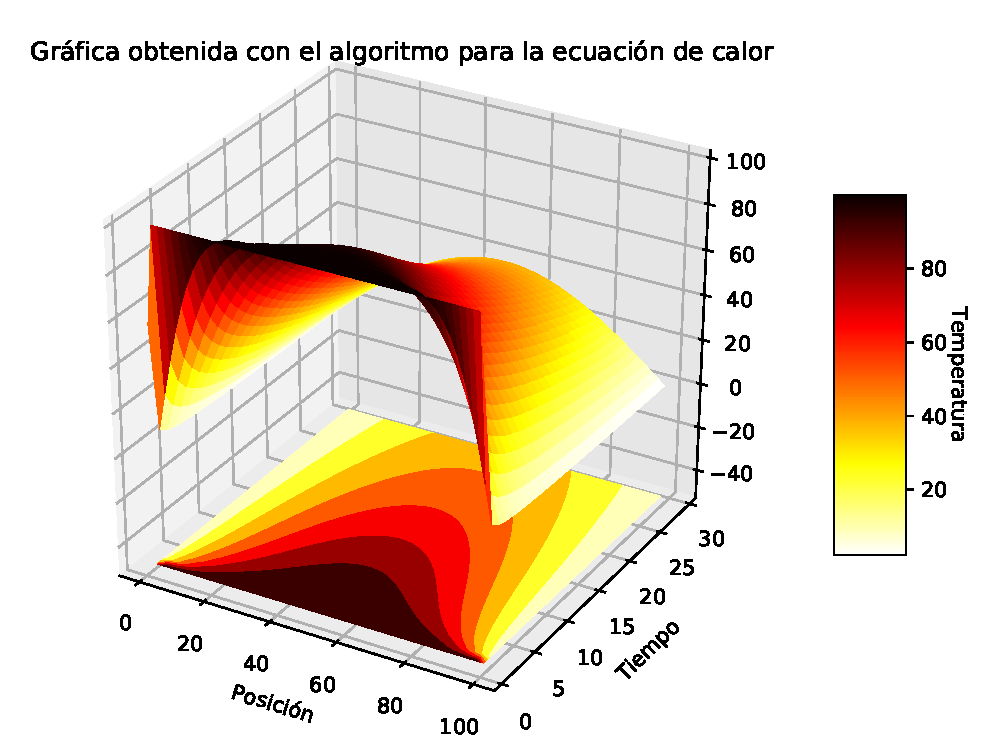
\includegraphics[scale=0.55]{Imagenes/SolucionEcuacionCalor_01.eps}  
\end{figure}
\end{frame}
}
\section{Problemas a resolver a cuenta de examen}
\begin{frame}
\frametitle{Problemas a resolver}
Se hacen algunos cambios en el planteamiento del problema, pero el algoritmo que hay que usar es el mismo, hay que resolver los siguientes casos:
\setbeamercolor{item projected}{bg=red!70!black,fg=white}
\setbeamertemplate{enumerate items}[circle]
\begin{enumerate}[<+->]
\item Distribución inicial de temperatura de forma senoidal: $\sin( \pi x / L)$
\item Dos barras en contacto cada una con diferente temperatura.
\item Modificación de la ecuación de calor para incluir un término y obtener la ley de enfriamiento de Newton.
\end{enumerate}
\end{frame}
\subsection{Problema 1}
\begin{frame}
\frametitle{Problema 1}
Distribución inicial de temperatura de forma senoidal: $\sin( \pi x / L)$
\\
\bigskip
Utiliza las mismas constantes que en el primer ejemplo. Puedes comparar los resultados con la solución analítica:
\[ T(x,t) = \sin \left( \dfrac{\pi \: x}{L} \right) \: \exp \left(-\dfrac{\pi^{2} \: R \: t}{L^{2}} \right), \hspace{0.75cm} R=\dfrac{K}{C \: \rho} \]
\end{frame}
\begin{frame}
\frametitle{Solución del problema 1}
\begin{figure}
	\centering
	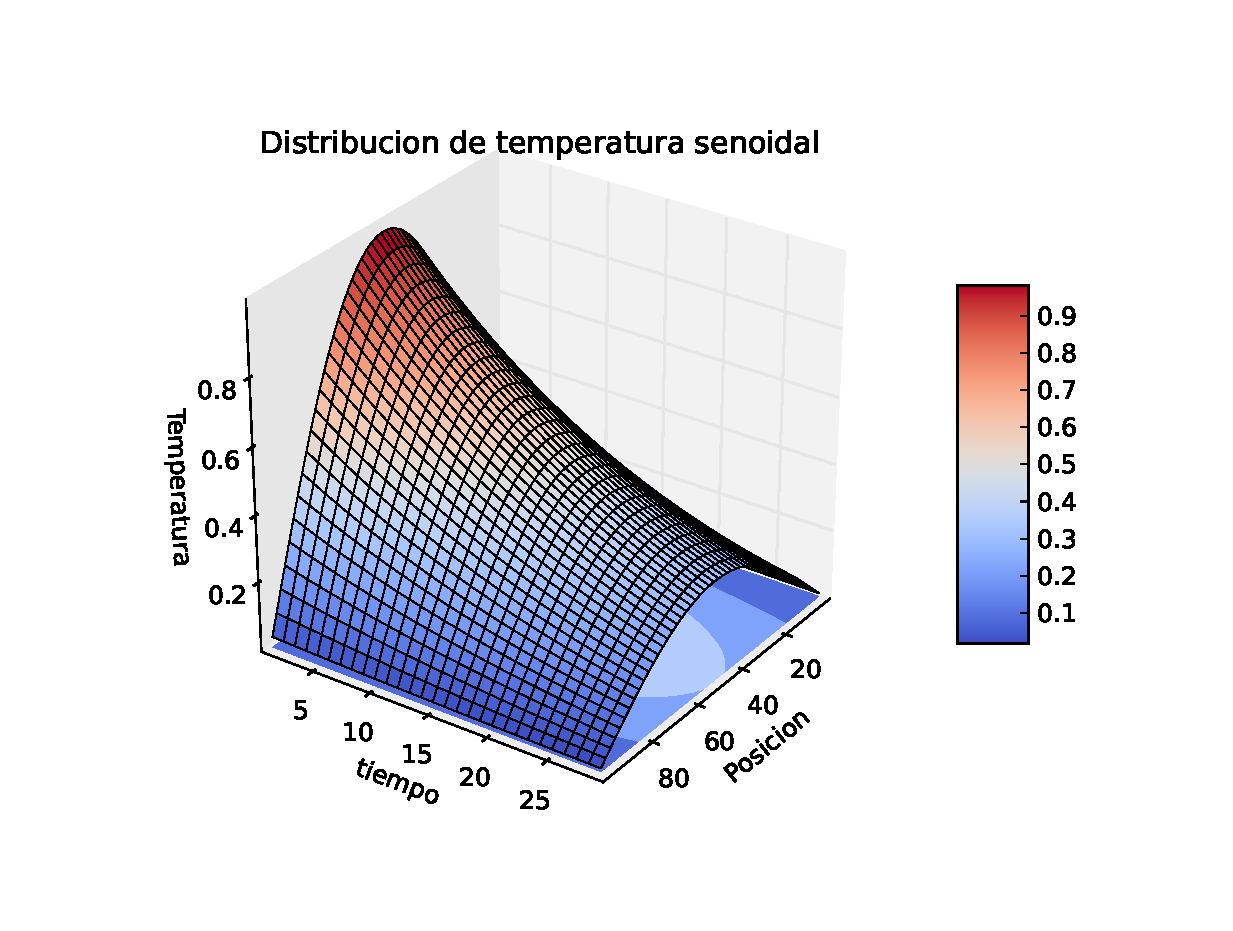
\includegraphics[scale=0.5]{Imagenes/EqCalor04.eps}  
\end{figure}
\end{frame}
\begin{frame}
\frametitle{Solución del problema 1 -rotada-}
\begin{figure}
	\centering
	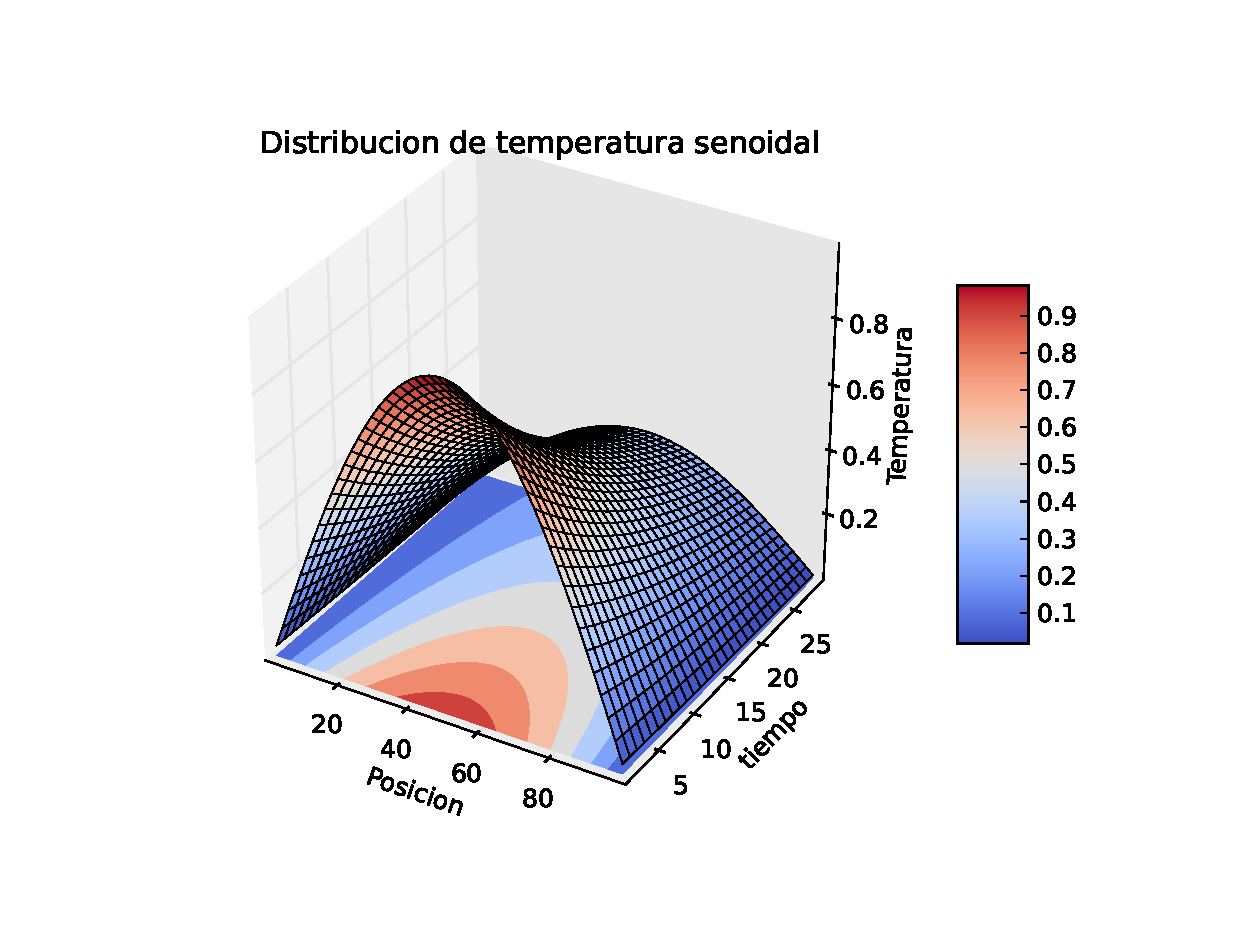
\includegraphics[scale=0.5]{Imagenes/EqCalor05.eps}  
\end{figure}
\end{frame}
\subsection{Problema 2}
\begin{frame}
\frametitle{Problema 2}
Tenemos dos barras del mismo material en contacto, cada una de ellas a diferente temperatura.
\end{frame}
\begin{frame}
\frametitle{Problema 2}
Las barras miden  $50 \: \si\cm$ de longitud. Una de ellas se mantiene a una temperatura de $100 \: \si\celsius$ y la otra a $50 \si\celsius$, se ponen en contacto a lo largo de su eje, un extremo de cada barra se mantiene a $0 \: \si\celsius$.
\\
\bigskip
Determina cómo varía la temperatura con respecto a la posición y al tiempo.
\end{frame}
\begin{frame}
\frametitle{Dos barras con diferente temperatura en contacto}
\begin{figure}
	\centering
	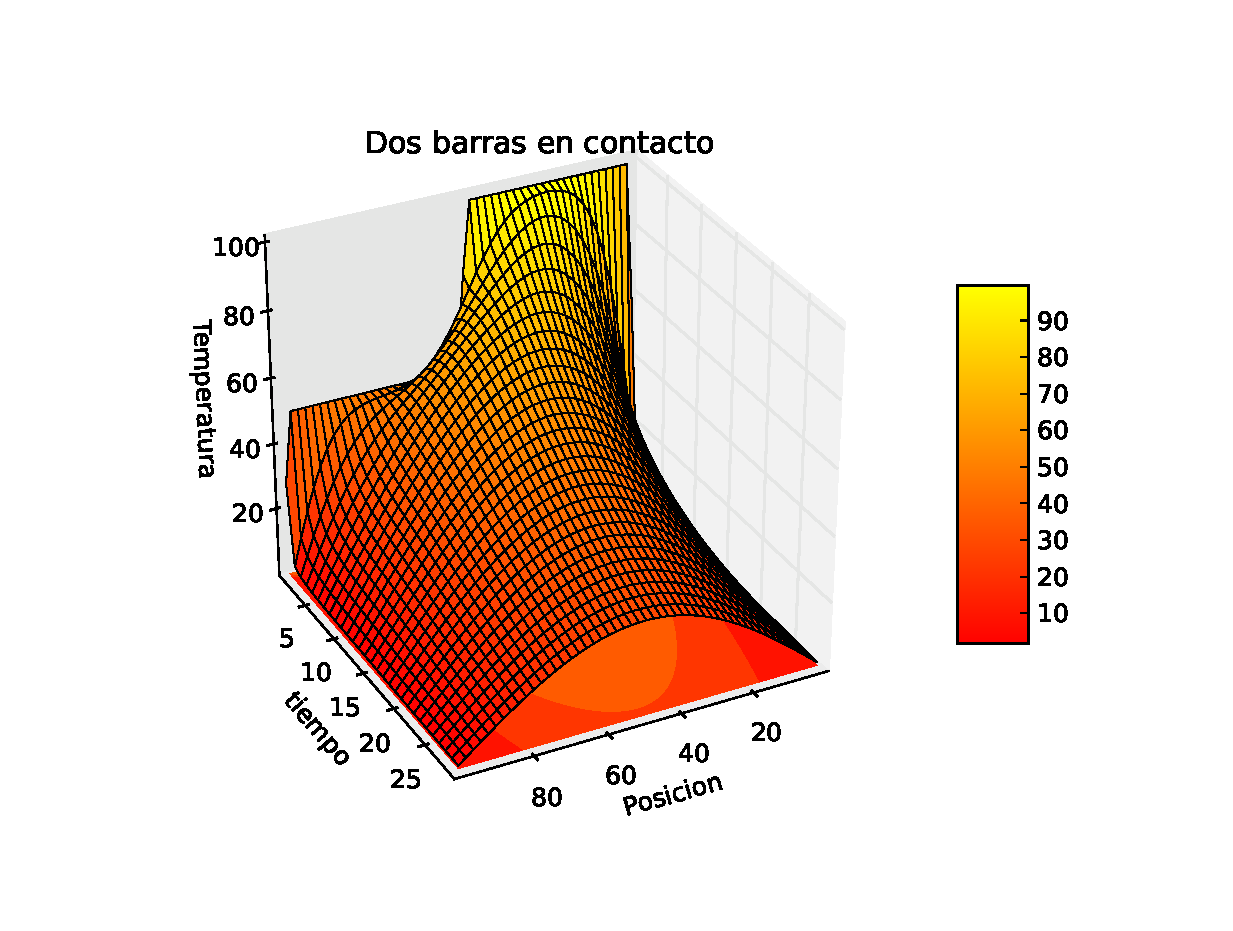
\includegraphics[scale=0.5]{Imagenes/EqCalor06.eps}  
\end{figure}
\end{frame}
\begin{frame}
\frametitle{Dos barras en contacto -rotada-}
\begin{figure}
	\centering
	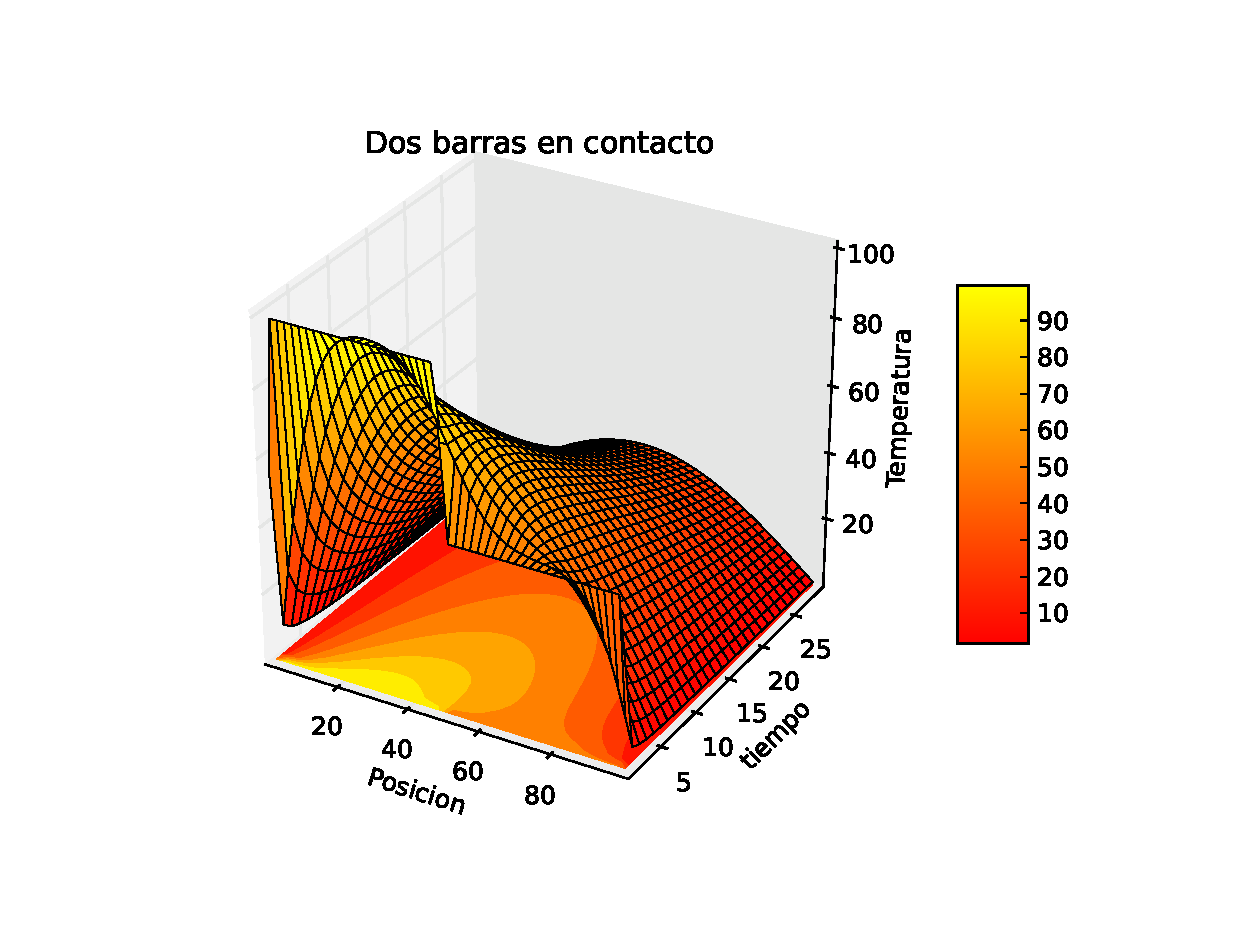
\includegraphics[scale=0.5]{Imagenes/EqCalor07.eps}  
\end{figure}
\end{frame}
\subsection{Problema 3}
\begin{frame}
\frametitle{Problema 3}
Modificación de la ecuación de calor para incluir un término y obtener la ley de enfriamiento de Newton.
\end{frame}
\begin{frame}
\frametitle{Problema 3}
Imagina ahora que la barra que estaba aislada (el problema con el que comenzamos la clase), se deja en contacto con el ambiente que se encuentra a una temperatura $T_{e}$, tal que es diferente a la temperatura inicial de la barra.
\end{frame}
\begin{frame}
\frametitle{Problema 3}
La ley de enfriamiento de Newton nos dice que la razón de cambio de la temperatura debido a la radiación es:
\[ \dfrac{\partial T}{\partial t} = - h (T- T_{e}) \]
\end{frame}
\begin{frame}
La ecuación de calor se modifica, quedando:
\[ \dfrac{\partial T(x,t)}{\partial t} = \dfrac{K}{C \: \rho} \dfrac{\partial^{2}T}{\partial x^{2}} - h \: T(x,t)\]
Ajusta el algoritmo y el programa para introducir el término de enfriamiento de Newton a lo largo de la barra. Compara el enfriamiento de esta barra con el ejemplo de la barra aislada.
\end{frame}
\begin{frame}
\frametitle{Barra aislada}
\begin{figure}
	\centering
	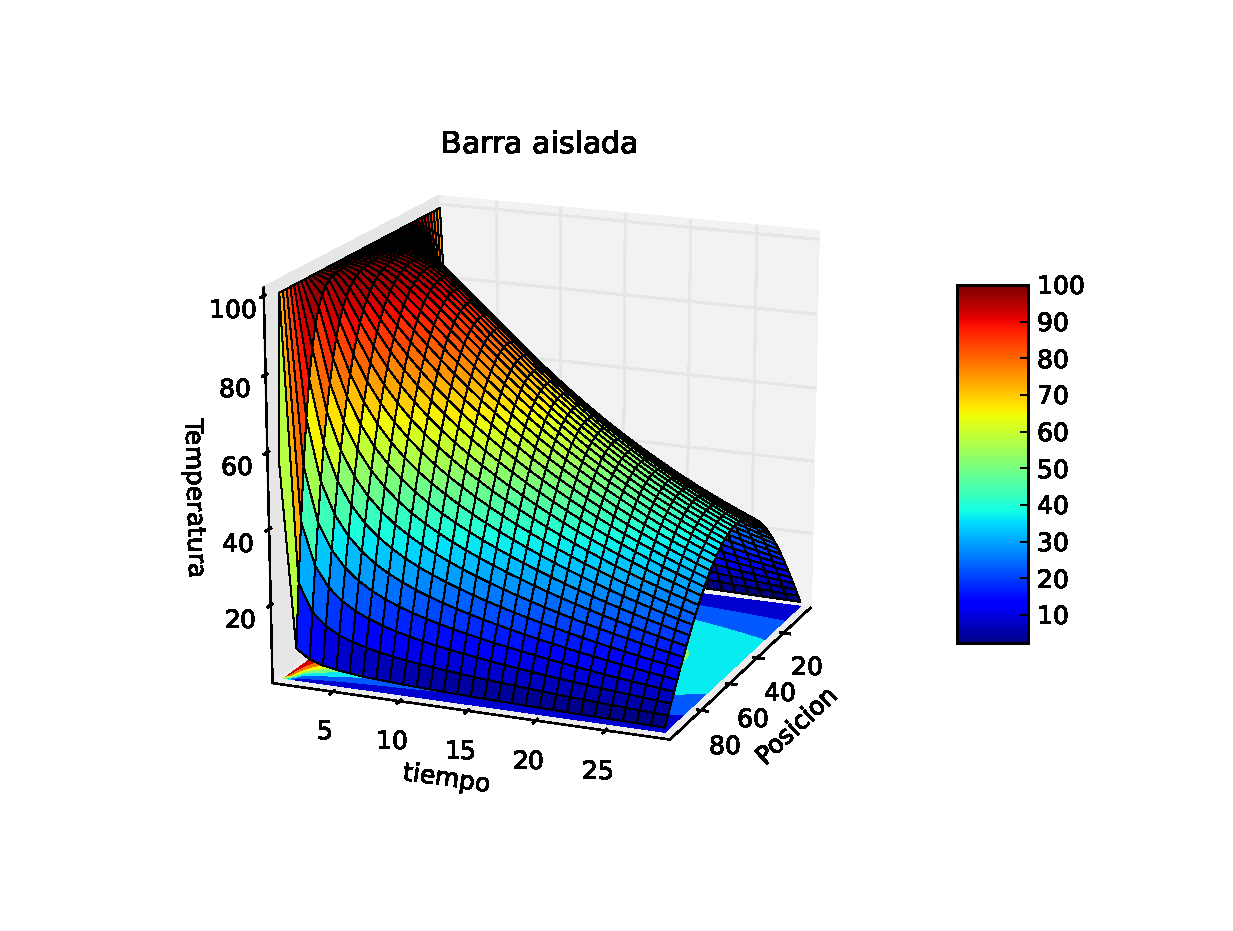
\includegraphics[scale=0.5]{Imagenes/EqCalor08.eps}  
\end{figure}
\end{frame}
\begin{frame}
\frametitle{Ley de enfriamiento de Newton, con $T_{e}=25 \si\celsius$}
\begin{figure}
	\centering
	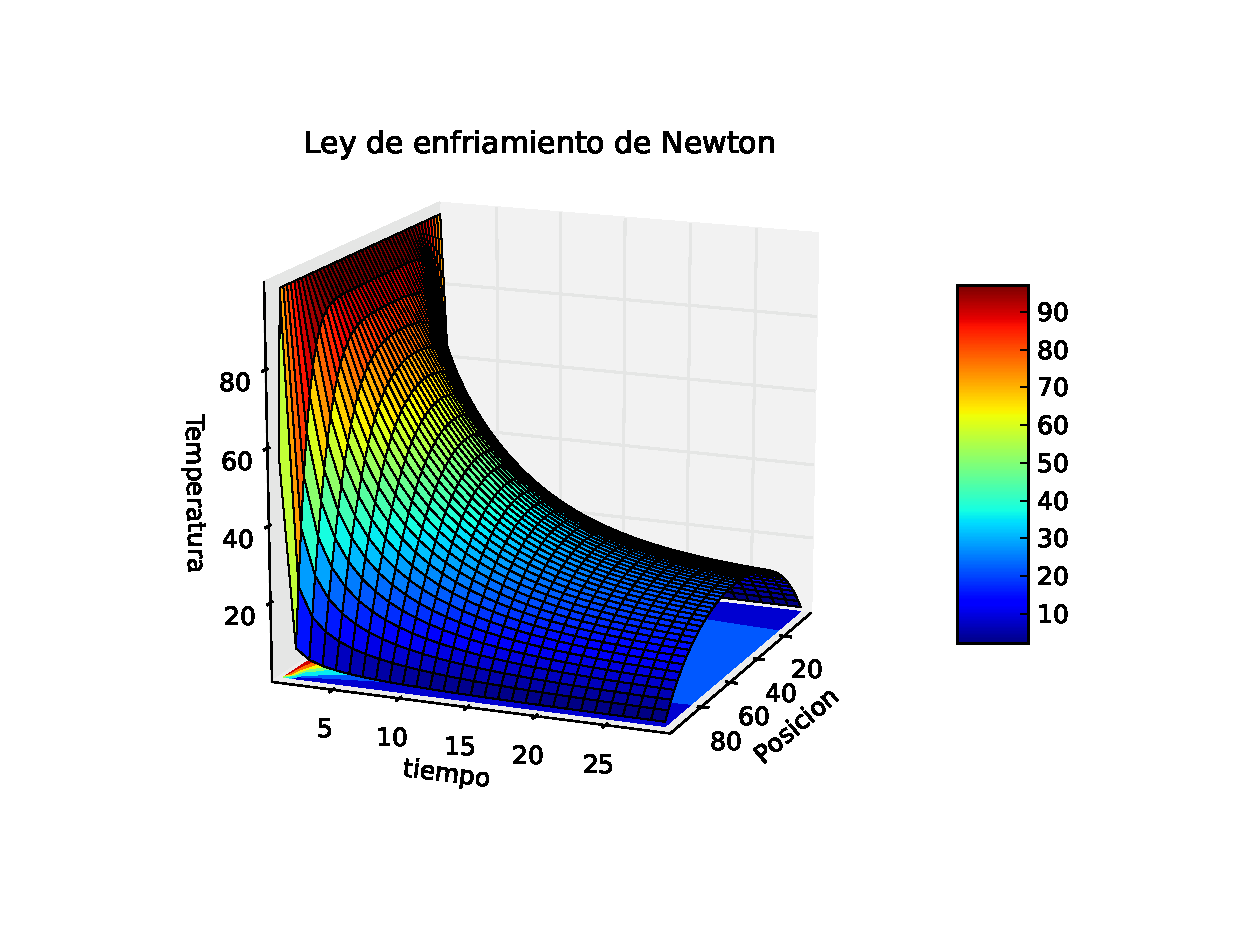
\includegraphics[scale=0.5]{Imagenes/EqCalor09.eps}  
\end{figure}
\end{frame}
\end{document}
